\documentclass[border=3mm]{standalone}

\usepackage{tikz}
\usetikzlibrary{arrows,shapes.gates.logic.US,shapes.gates.logic.IEC,calc}
\begin{document}
\thispagestyle{empty}
\tikzstyle{branch}=[fill,shape=circle,minimum size=3pt,inner sep=0pt]
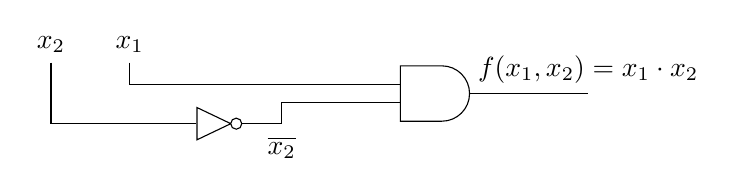
\begin{tikzpicture}[label distance=2mm]

    \node (x2) at (0,0) {$x_2$};
    \node (x1) at (1,0) {$x_1$};


    \node[not gate US, draw, minimum size=10pt] at ($(x2)+(2,-1)$) (Not1) {};

    \node[and gate US, draw, logic gate inputs=nn, anchor=input 1, minimum size=20pt] at ($(Not1.output)+(2,0.5)$) (And1) {};

      \draw (x1) |- (And1.input 1);
      \draw (x2) |- (Not1.input);
      \draw (Not1.output) -- ([xshift=0.5cm]Not1.output)  |- (And1.input 2) node[near start, below=5pt] {$\overline{x_2}$};
      \draw (And1.output) -- ([xshift=1.5cm]And1.output) node[above] {$f(x_1,x_2) = x_1 \cdot x_2$};

\end{tikzpicture}
\end{document} 
